
\section{The Point-To-Point mesh}


\subsection{\label{sub:Architecture}Architecture}

The NS-3 simulator is heavily based on object-oriented design. Figure
\ref{fig:singlehop} shows a simplified view on a typical NS-3 simulation
architecture, regardless whether programmed in Python or C++.

%
\begin{figure}
\begin{centering}
% Define two helper counters
\begin{tikzpicture}[auto]

   % % grid
   % \def\supertiny{ \font\supertinyfont = cmr9 at 3pt \relax \supertinyfont}
   % \newcounter{gridrows}
   % \setcounter{gridrows}{12}
   % \newcounter{gridcols}
   % \setcounter{gridcols}{30}
   % \draw [gray, very thin] (0, -\arabic{gridrows}) grid (\arabic{gridcols}, 0);
   % \foreach \x in {0,...,\arabic{gridcols}}
   %     \foreach \y in {0,...,\arabic{gridrows}}
   %     {
   %         \draw (\x+0.15, -\y-0.15) node [gray, very thin] {\supertiny{\x/\y}};
   %     }

    % styles
    \tikzstyle{archlayer} = [
        shape=rectangle, 
        draw, 
        rounded corners=2pt, 
        inner sep=0mm, 
        minimum width=30mm, 
        minimum height=10mm,
        fill=blue!20
    ];

    \tikzstyle{darrow} = [latex-latex];

    \node[archlayer] (app) {Application};
    \node[archlayer, fill=yellow!20, below=of app] (stack) {Protocol stack};
    \path (app) edge[darrow] (stack);
    \node[archlayer, fill=green!20, below=of stack] (netdevice) {NetDevice};
    \path (stack) edge[darrow] (netdevice);

    \node[archlayer, fill=red!20, right=of netdevice] (channel) {Channel};
    \path (netdevice) edge[darrow] (channel);

    \node[archlayer, fill=green!20, right=of channel] (netdevice) {NetDevice};
    \path (channel) edge[darrow] (netdevice);
    \node[archlayer, fill=yellow!20, above=of netdevice] (stack) {Protocol stack};
    \path (netdevice) edge[darrow] (stack);
    \node[archlayer, above=of stack] (app) {Application};
    \path (app) edge[darrow] (stack);
\end{tikzpicture}

\par\end{centering}

\caption{Typical NS-3 simulation architecture}



\end{figure}


The following architectual layers can be identified:
\begin{itemize}
\item \textit{Application}: This layer contains the application logic. In
NS-3 one can implement socket-based applications using the internal
NS-3 socket APIs. NS-3 actually also provides operating system dependent
socket implementations (as far as I know the Linux socket API and
the BSD API is supported in NS-3). Finally UDP based applications
are supported and also various helper classes are provided by NS-3
for easy initialization of the application objects. The current project
focuses only on UDP based applications.
\item \textit{Protocol stack}: This architectual layer provides objects
for initializing a concrete protocol stack. Since NS-3 currently only
supports IPv4 only this is the stack the current project relies on.
Furthermore on this layer one specifies the different routing mechanisms
being used by NS-3. The current project uses both supported routing
protocols (static routing and OLSR).
\item \textit{NetDevice}: This layer provides objects for defining the actual
physical layout of the network. In the current project physically
Point-To-Point connections are being examined as well as Wifi connections.
Furthermore this layer provides objects for specifying the actual
positions and movements for the nodes of interest.
\item \textit{Channel}: This layer provides objects the physical communication
channel between nodes. This layer is pretty much hidden from the developer
but hooks and callback methods exists for further analysis and statistics.
\end{itemize}

\subsection{Single Hop simulation}

%
\begin{figure}
\begin{centering}
% Define two helper counters
\begin{tikzpicture}[auto]

   % % grid
   % \def\supertiny{ \font\supertinyfont = cmr9 at 3pt \relax \supertinyfont}
   % \newcounter{gridrows}
   % \setcounter{gridrows}{12}
   % \newcounter{gridcols}
   % \setcounter{gridcols}{30}
   % \draw [gray, very thin] (0, -\arabic{gridrows}) grid (\arabic{gridcols}, 0);
   % \foreach \x in {0,...,\arabic{gridcols}}
   %     \foreach \y in {0,...,\arabic{gridrows}}
   %     {
   %         \draw (\x+0.15, -\y-0.15) node [gray, very thin] {\supertiny{\x/\y}};
   %     }

    % styles
    \tikzstyle{netnode} = [shape=rectangle, draw, rounded corners=2pt, fill=black!20, minimum height=10mm, minimum width=30mm];
    \tikzstyle{darrow} = [latex-latex];

    \draw 
        node[netnode] (node1) {Node 1}
        node[netnode, right=of node1, xshift=3cm] (node2) {Node 2};

    \path
        (node1) edge[darrow] node{Point-To-Point} node[swap]{500kbs, 2ms Delay} (node2);
\end{tikzpicture}

\par\end{centering}

\caption{\label{fig:singlehop}Point-To-Point connection between two nodes}

\end{figure}


The first simulation analyzes two nodes being connected together via
a Point to Point connection. Figure \ref{fig:singlehop} represents
the very simple network being simulated in this case. Listing \ref{lst:singlehop}
shows the relevant Python based program code for this simulation.\texttt{\small \lstinputlisting[breaklines=true,caption={experiment.py (singleHop simulation)},extendedchars=true,firstline=60,label={lst:singlehop},language={Python},lastline=92,numbers=right]{src/sieci/src/experiment.py}}{\small \par}

First a NodeContainer object is being created which instantiates all
simulated nodes of the target network. Afterwards follows a DeviceFactory
which was implemented individually for this project. It initializes
and creates the actual physical devices. Listing \ref{lst:devfactory}
shows the relevant initalization code. One can see that a Point-To-Point
connection between the nodes having a speed of 500kbs and a delay
of 2ms is being initialized.

\texttt{\small \lstinputlisting[breaklines=true,caption={experiment.py (DeviceFactory initialization)},extendedchars=true,firstline=5,label={lst:devfactory},language={Python},lastline=11,numbers=right]{src/sieci/src/experiment.py}}{\small \par}

Afterwards the internet protocol stack is being initialized using
internal NS-3 helper objects. The most important part here is the
assignment of IP addresses to the simulated nodes which is also being
handled by a helper object. Only a base address (here {}``10.0.0.0'')
has to be specified and NS-3 will chronologically assign IP addresses
automatically to all simulated nodes. Here we have two nodes, therefore
the adresses {}``10.0.0.1'' and {}``10.0.0.2'' will be assigned
to the nodes.

At last the actual applications are being initialized using an application
factory developed individually for of this project. The initialization
in Listing \ref{lst:appfactory} install two applications, the sender
application (tx) and the receiver application (rx). Using NS-3 helper
objects an UDP based application is instanciated, which is sending
packets starting at OnTtheime and stopping at OffTime. Here the application
starts sending packets after 1 second of the application start and
never stops sending (OffTime is 0 seconds).

\texttt{\small \lstinputlisting[breaklines=true,caption={experiment.py (ApplicationFactory initialization)},extendedchars=true,firstline=34,label={lst:appfactory},language={Python},lastline=58,numbers=right]{src/sieci/src/experiment.py}}{\small \par}

Since this network consists of only two nodes, it is not necessary
to initialize any routing tables. The two nodes see each other directly.
Python based logging statements were built into the singlehop simulation
and the output can be seen in Listing \ref{lst:singlehoplog}. The
log shows the assigned MAC addresses as well as the dynamically assigned
IP addresses of both nodes.

\texttt{\small \lstinputlisting[breaklines=true,caption={singlehop.log (SingleHop simulation log output)},extendedchars=true,label={lst:singlehoplog}]{src/results/singlehop.log}}{\small \par}

In line 82 and line 84 of lising \ref{lst:singlehop} one can see
that the receiver application starts listening for UDP packets 15
seconds after the beginning of the simulation. The sender application
starts sending UDP packets 5 seconds earlier at the 10th second after
the simulation start. What happens then can be seen best from the
actual packet traces generated by NS-3. It is capable of generating
standard pcap based output files. The pcap trace file can then be
analyzed using existing tools available (i.e. tcpump, wireshark, tcptrace,
etc.). The tcpdump of the generated pcap files can be seen in listing
\ref{lst:singlehoptcpdump}. It can be seen that as long as the receiver
application is not listening for any packets, an ICMP message is being
answered from the receiver node, stating that the application port
is unreachable. Starting from the 15th second the receiver application
then silently accepts the incoming UDP packets.

\texttt{\small \lstinputlisting[breaklines=true,caption={singlehop.tcpdump (SingleHop tcpdump output)},extendedchars=true,label={lst:singlehoptcpdump}]{src/results/singlehop.tcpdump}}{\small \par}


\subsection{Dual Hop simulation using OLSR}

Using the same code basis from the single hop simulation a further
simulation was developed to examine NS-3's routing table capabilities.
Listing \ref{lst:dualhop_} shows the relevant code fragments. The
simulated network consists of three nodes as represented in figure
\ref{fig:Point-To-Point-connection-between}. The nodes are connected
together using a Point-To-Point connection. One can see, that Node1
and Node3 do not see each other physically. Instead Node2 is initialized
to have two net devices, one connecting to Node1 and the other connecting
to Node3. Thus Node1 and Node3 are transiently connected via Node2.
A routing protocol is needed to successfully propagate any packets
from Node1 to Node3. Lines 140-141 of listing \ref{lst:dualhop_}
show the correspondent OLSR initialization code under NS-3.

Because OLSR needs some time to initialize the start of the sender
application and the receiver application were delayed to the 70th
second (sender) and the 80th second (receiver). If the sender starts
too early, the routing tables would not be initialized yet causing
unroutable packets. That is actually one drawback of dynamic routing
protocols. They need time to build and need time to update themself
by a certain delay.

\texttt{\small \lstinputlisting[breaklines=true,caption={experiment.py (dualHop simulation)},extendedchars=true,firstline=94,label={lst:dualhop_},language={Python},lastline=150,numbers=right]{src/sieci/src/experiment.py}}{\small \par}

For the analysis of the dual hop simulation wireshark has been used
because of its very detailed information depth. NS-3 generates a pcap
file for each net device so for the dual hop simulation the following
pcap files exist:

\begin{center}
\begin{tabular}{|c|c|}
\hline 
Node & pcap files\tabularnewline
\hline
\hline 
Node 1 & \multicolumn{1}{c|}{dualHopOlsr-0-0.pcap}\tabularnewline
\hline 
Node 2 & dualHopOlsr-1-0.pcap\tabularnewline
 & dualHopOlsr-1-1.pcap\tabularnewline
\hline 
Node 3 & dualHopOlsr-2-0.pcap\tabularnewline
\hline
\end{tabular}
\par\end{center}

One can see that Node 2 has two pcap files, one for each of the two
assigned net devices forming a Point-To-Point connection with Node
1 on one side and Node 2 an the other. Listing \ref{lst:dualhop_wireshark}
shows the first two packets from the dualHopOlsr-1-0.pcap file, which
represents the channel between Node 1 (10.0.1.1) and Node 2 (10.0.1.2).
The shown two packets are so called HELLO packets. This message type
is defined in the OLSR RFC \cite{rfc3626} as the message type to
propagate the information that a node is actually existent in the
network. All receiving nodes (at least those who are capable of receiving
these HELLO messages) will then know of the existence of the neighbour
nodes and can build a routing table based on this information. Another
interesting fact is the usage of the MID (Multiple Interface Declaration)
message type in the second packet. This message type is used, when
a node has multiple interfaces, which is the case for Node 2. \texttt{\small \lstinputlisting[breaklines=true,caption={dualHopOlsr-1-0.log (dualHop wireshark dump)},extendedchars=true,label={lst:dualhop_wireshark}]{src/results/dualHopOlsr-1-0.log}}{\small \par}

Figure \ref{fig:IO-Graph-statistics} shows the IO graph of the dual
hop simualation, generated using wireshark. Line 132 and line 133
in Listing \ref{lst:dualhop_} specify that the sender application
is supposed to start transmitting UDP packets from the 80th second
up to the 90th second after the simulation start. This peak of packet
activity can be nicely observed in Figure \ref{fig:IO-Graph-statistics}.
A further observation is that when the application is not sending
data, there is still packet traffic existent. It is visible as small
spikes in the IO graph. When observing the wireshark trace then it
can be concluded that this is traffic generated by the OLSR protocol.
So one can say that OLSR is a proactive routing protocol which constantly
updates himself. There is no need for an external {}``trigger''
which initializes the routing update. Therefore this routing protocol
is also suitable for moving nodes, where neighbour nodes change constantly
and thus also the routing information.

%
\begin{figure}
\begin{centering}
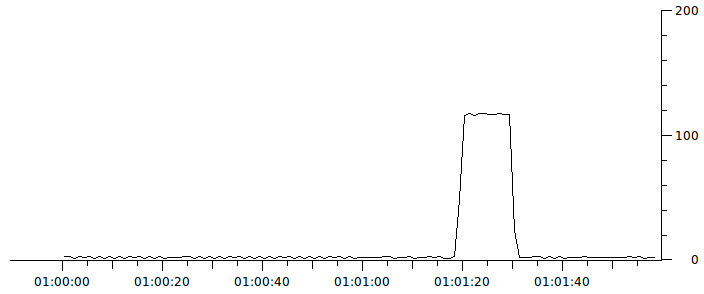
\includegraphics[width=0.7\paperwidth]{src/results/dualHopOlsr}
\par\end{centering}

\caption{\label{fig:IO-Graph-statistics}IO Graph statistics of the dual hop
simulation}

\end{figure}

